\documentclass[10pt,a4paper,landscape]{article}
\usepackage[margin=15mm,headheight=14pt,headsep=5mm,footskip=8mm]{geometry}
\usepackage[T1]{fontenc}
\usepackage{lmodern,microtype,xcolor,tikz,tabularx,booktabs,array,fancyhdr,hyperref}
\usetikzlibrary{arrows.meta,positioning}
\renewcommand{\familydefault}{\sfdefault}
\definecolor{navy}{HTML}{183447}
\definecolor{teal}{HTML}{147B80}
\definecolor{pale}{HTML}{EDF6F5}
\definecolor{slate}{HTML}{526574}
\definecolor{rulegray}{HTML}{CDDDE2}
\definecolor{sand}{HTML}{FCF3E4}
\hypersetup{colorlinks=true,urlcolor=teal,pdftitle={Financial news prediction: progress meeting brief},pdfauthor={Research progress report}}
\pagestyle{fancy}\fancyhf{}
\fancyhead[L]{\small\color{slate}FINANCIAL NEWS / RESEARCH PROGRESS}
\fancyhead[R]{\small\color{slate}14 OCTOBER 2026}
\fancyfoot[L]{\scriptsize\color{slate}Public-data FININ-inspired adaptation / exploratory evidence}
\fancyfoot[R]{\small\color{slate}\thepage\ / 2}
\renewcommand{\headrulewidth}{0pt}
\setlength{\parindent}{0pt}\setlength{\parskip}{5pt}
\renewcommand{\arraystretch}{1.15}\setlength{\tabcolsep}{7pt}
\newcolumntype{Y}{>{\raggedright\arraybackslash}X}
\newcommand{\heading}[1]{{\fontsize{23}{27}\selectfont\bfseries\color{navy}#1}\par}
\newcommand{\sub}[1]{\vspace{3pt}{\large\bfseries\color{navy}#1}\par}
\newcommand{\callout}[1]{\par\colorbox{pale}{\parbox{\dimexpr\linewidth-2\fboxsep}{\vspace{4pt}#1\vspace{4pt}}}\par}
\newcommand{\caution}[1]{\par\colorbox{sand}{\parbox{\dimexpr\linewidth-2\fboxsep}{\vspace{4pt}#1\vspace{4pt}}}\par}
\tikzset{box/.style={draw=rulegray,rounded corners=3pt,align=center,text width=4.2cm,minimum height=1.8cm,inner sep=5pt,font=\small,text=navy},core/.style={box,fill=pale,draw=teal},arr/.style={-{Stealth[length=2mm]},line width=.8pt,draw=slate}}
\begin{document}

\heading{A working testbed; useful news forecasts remain unproven}
\textbf{Research focus:} does news retain forecasting value as it gets older, and does explicit age weighting help?
\callout{\textbf{Progress:} built and audited a public company-news pipeline, then completed two controlled temporal comparisons. \textbf{Neither established a meaningful forecasting benefit.}}

{\small\color{slate}\textbf{Since the first brief:} NIFTY-news/SPY prototype $\rightarrow$ StockNet and SPNews adaptations $\rightarrow$ current CMIN-US company panel. Earlier experiments and negative results are preserved. This is an independent adaptation, not an empirical reproduction of FININ.}

\sub{Current pipeline: the pooled version used in the recent tests}
\begin{center}
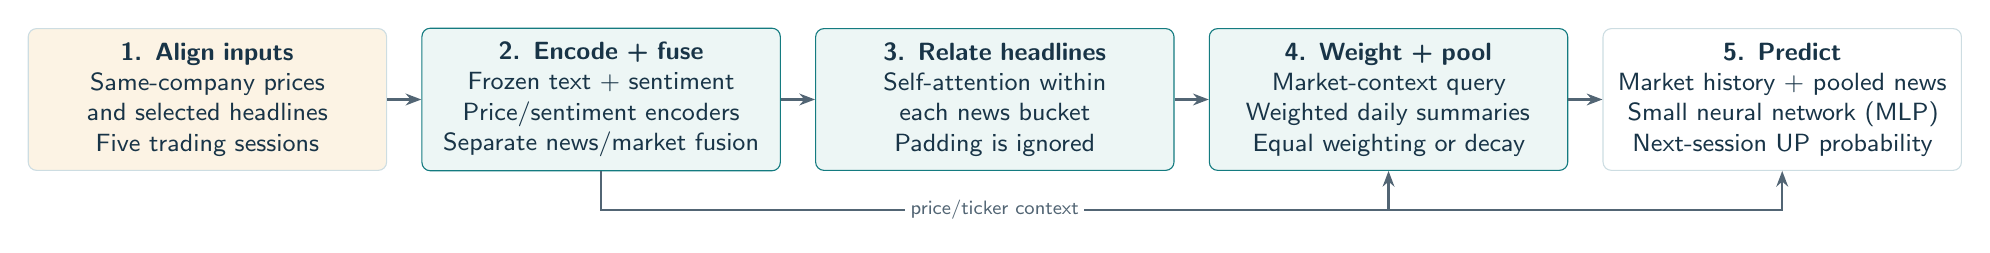
\begin{tikzpicture}[x=1cm,y=1cm]
\node[box,fill=sand] (p1) at (0,0) {\textbf{1. Align inputs}\\Same-company prices\\and selected headlines\\Five trading sessions};
\node[core] (p2) at (5,0) {\textbf{2. Encode + fuse}\\Frozen text + sentiment\\Price/sentiment encoders\\Separate news/market fusion};
\node[core] (p3) at (10,0) {\textbf{3. Relate headlines}\\Self-attention within\\each news bucket\\Padding is ignored};
\node[core] (p4) at (15,0) {\textbf{4. Weight + pool}\\Market-context query\\Weighted daily summaries\\Equal weighting or decay};
\node[box] (p5) at (20,0) {\textbf{5. Predict}\\Market history + pooled news\\Small neural network (MLP)\\Next-session UP probability};
\foreach \a/\b in {p1/p2,p2/p3,p3/p4,p4/p5}{\draw[arr](\a)--(\b);}
\draw[arr] (p2.south)--(5,-1.4)--(15,-1.4)--(p4.south);
\draw[arr] (15,-1.4)--(20,-1.4)--(p5.south);
\node[font=\scriptsize,text=slate,fill=white,inner sep=2pt] at (10,-1.4) {price/ticker context};
\end{tikzpicture}
\end{center}
{\small\textbf{Before the final MLP:} five market vectors (80 values) + one pooled news vector (16 values) = \textbf{96 inputs}. Fused prices/ticker context supplies the market query and also feeds the predictor. Sentiment joins each headline earlier; weights shape the summary rather than becoming extra columns. The initial baseline used 160 concatenated inputs; these tests match the pooled geometry.}

\begin{minipage}[t]{.49\linewidth}
\sub{Inputs, in plain language}
\textbf{News:} company-linked headline titles; at most six per arrival session, up to 30 across the history. Frozen sentiment gives positive, neutral and negative scores.\par
\textbf{Market:} six price/volume features per session, plus a fixed company-ticker text description. No future prices enter the inputs.\par
{\small\color{slate}\textbf{Frozen:} RoBERTa text and finance TinyBERT sentiment. \textbf{Trained:} projection, numeric/fusion layers, attention and predictor.}
\end{minipage}\hfill
\begin{minipage}[t]{.47\linewidth}
\sub{Evidence available}
\textbf{12 companies; 9,984 eligible company-days.}\par
\textbf{2,004 evaluated cases on 167 market dates.}\par
Two chronological evaluation periods: May--August 2020 and January--April 2021; two random initializations per model.\par
{\small\color{slate}Coverage is uneven; one company has no development news. Company-days on the same market date are not independent.}
\end{minipage}

\sub{One forecast: what is known, and when?}
\begin{center}

\begin{tikzpicture}
\node[box,text width=4.8cm,minimum height=1cm] (n) at (0,0) {\textbf{Source news date $D$}\\Exact publication time uncertain};
\node[box,fill=sand,text width=4.8cm,minimum height=1cm] (a) at (6.2,0) {\textbf{Assume availability at $D+2$}\\Two calendar days, midnight UTC};
\node[core,text width=4.8cm,minimum height=1cm] (d) at (12.4,0) {\textbf{Forecast at close $d$}\\Use eligible news and prices};
\node[box,text width=4.8cm,minimum height=1cm] (q) at (18.6,0) {\textbf{Answer at next close $q$}\\Did adjusted close increase?};
\foreach \x/\y in {n/a,a/d,d/q}{\draw[arr](\x)--(\y);}
\end{tikzpicture}
\end{center}
{\small\color{slate}News enters its first eligible exchange-close bucket. In an ordinary trading week: Monday source date $\rightarrow$ Wednesday forecast $\rightarrow$ Thursday answer. This delay is a timing assumption, \textbf{not verified historical availability}; the relevant information may already be priced in.}

\newpage
\heading{What was tested, and what can we report?}
\begin{minipage}[t]{.49\linewidth}
\sub{Test A / Does explicit decay help?}
Keep the same news, five-session price history and model geometry. Compare equal temporal weighting with a \textbf{48-hour half-life}: each extra 48 hours halves a story's multiplier, before normalization.\par
\textbf{Result:} a tiny loss reduction of \textbf{0.000324}; the uncertainty interval includes both improvement and worsening. No practical benefit was established.\par
{\small\color{slate}Eight fits. The age-removal curve was tiny and non-monotone; it did not identify a market decay law.}
\end{minipage}\hfill
\begin{minipage}[t]{.47\linewidth}
\sub{Test B / Does older news add value?}
Keep five price sessions in every model. Compare prices only, prices + the \textbf{current arrival bucket}, and prices + current and four older buckets.\par
\textbf{Result:} adding older news \textbf{increased loss by 0.000560} on average. Seeds disagreed; no useful older-news addition was established.\par
{\small\color{slate}Eight new fits; four matching all-news fits reused. ``Current'' means proxy arrival, not verified fresh publication.}
\end{minipage}

\sub{Scores on the same evaluation dates}
\begin{tabularx}{\linewidth}{@{}YrY@{}}
\toprule
\textbf{Model / reference} & \textbf{Log loss} & \textbf{How to read the result}\\\midrule
Constant training-prevalence probabilities & 0.689820 & Reference using no daily news or price changes\\
Prices only (matched pooled model) & 0.689771 & Almost the same as the constant reference\\
Prices + current news bucket & 0.689651 & Lowest point estimate; advantage is tiny and uncertain\\
Prices + current and older news, equal weighting & 0.690210 & Older-news addition did not improve forecasting\\
Prices + current and older news, 48-hour decay & 0.689887 & Tiny change; no reliable decay benefit\\
\bottomrule
\end{tabularx}\par
{\small\textbf{Log loss measures probability quality; lower is better.} Results average model losses across two initializations, not an ensemble. The predeclared practical improvement was 0.005; neither temporal test met it.}

\begin{minipage}[t]{.49\linewidth}
\sub{What is verified}
The implementation consumes news: changing inputs can change predicted probabilities. Saved forecasts, timing rules, model states and comparisons were independently audited.\par
\textbf{Changing a prediction does not mean improving it.} Forecasts remained mostly UP; both later-period decay models predicted UP throughout.
\end{minipage}\hfill
\begin{minipage}[t]{.47\linewidth}
\sub{What remains unresolved}
Exact publication/availability times and some source-date conflicts. Whether weak results come from timing, relevance, representations, learning or weak predictability.\par
These periods were already inspected: the results are \textbf{exploratory}. The experiments do not establish causality, trading value or information diffusion.
\end{minipage}

\caution{\textbf{Meeting takeaway:} ``I tested explicit decay and older-news contribution using matched comparisons. Neither delivered a meaningful forecasting gain. I preserved the negative results and stopped further model variations.''}
\textbf{Decision for the next stage:} agree the data/timing standard and empirical question before another model. A timestamped earnings-release/movement-size approach was discussed only; it has \textbf{not been built or validated}.

\vfill
{\scriptsize\color{slate}\textbf{Evidence:} \texttt{reports/cmin\_news\_decay\_2026-10-14.md}; \texttt{reports/cmin\_older\_news\_2026-10-14.md}; their saved experiment artifacts and independent final reviews. Conditional 95\% loss-difference intervals: decay minus equal weighting $[-0.001176,\,+0.000539]$; all-news minus current news $[-0.000031,\,+0.001155]$. Date-block intervals retain companies together and omit training uncertainty.}\par
{\scriptsize\color{slate}\textbf{Reference:} Wang, Cohen \& Ma (2024), \href{https://aclanthology.org/2024.findings-emnlp.189/}{\emph{Modeling News Interactions and Influence for Financial Market Prediction}}, Sections 4.2--4.3 and 6.4. FININ has no explicit exponential decay term; this public-data study is an independent extension.}
\end{document}
